\index{Pfander, G\"otz}
\subsubsection{Applied Harmonic Analysis}\label{mps:pfander}

\paragraph{Research Team}
G\"otz Pfander (Professor), Niklas Grip (Postdoctoral Fellow), Peter Rashkov (PhD Student)

\medskip

One of the traditional goals in harmonic and functional analysis
is the development of efficient methods to assemble (synthesize)
or decompose (analyse) functions or operators into
well-understood basic building blocks. In recent years,
mathematical contributions to these objectives had a tremendous
impact on signal processing and communications engineering:
wavelet bases were designed to analyze images (jpeg2000), and
Gabor systems are currently used to transmit data through wired or
wireless channels.

Our research agenda is twofold. On the one hand, we seek to apply
methods from harmonic analysis to offer improvements to
communications systems (Section~\ref{ict:pfander}). On the other
hand, we use questions that arise in communications engineering as
stimulus to prove interesting mathematical theorems, which in many
cases are far removed from the interests and needs of
communications engineering. Results of this more theoretical
nature are described below.



%%%%%%%%%%%%%%%%%%%%%%%%%%%%%%%%%%%%%%%%%%%%%%%%%%%%%
%%%%%%%%%%%%%%%%%%%%%%%%%%%%%%%%%%%%%%%%%%%%%%%%%%%%%


\paragraph{Highlights}
This year's most important achievement  is the development of an
operator sampling theory. This theory, which is described below, is
based on previous results that were motivated by the channel
measurement problem in communcations engineering
\cite{KP06,PW06,PW06b} (Section~\ref{ict:pfander}).


%%%%%%%%%%%%%%%%%%%%%%%%%%%%%%%%%%%%%%%%%%%%%%%%%%%%%
%%%%%%%%%%%%%%%%%%%%%%%%%%%%%%%%%%%%%%%%%%%%%%%%%%%%%

\smallskip

{\sl Operator sampling:}
Shannon's classical sampling theorem states that a bandlimited
function can be recovered from its samples, as long as we use a
sufficiently dense sampling grid. In recent work, we widenened this
classical theorem, replacing functions by ``bandlimited operators'',
that is, by pseudodifferential operators which have bandlimited
Kohn-Nirenberg symbols. We show that such operators can be recovered
from their action on a distribution which is supported on a
sufficiently dense sampling grid if and only if the Kohn-Nirenberg
symbol of the operator is bandlimited to a set of area less than
one.


% to include a figure, generate a file xxx.pdf and integrate the following lines
\begin{figure}[ht]
  \begin{center}
   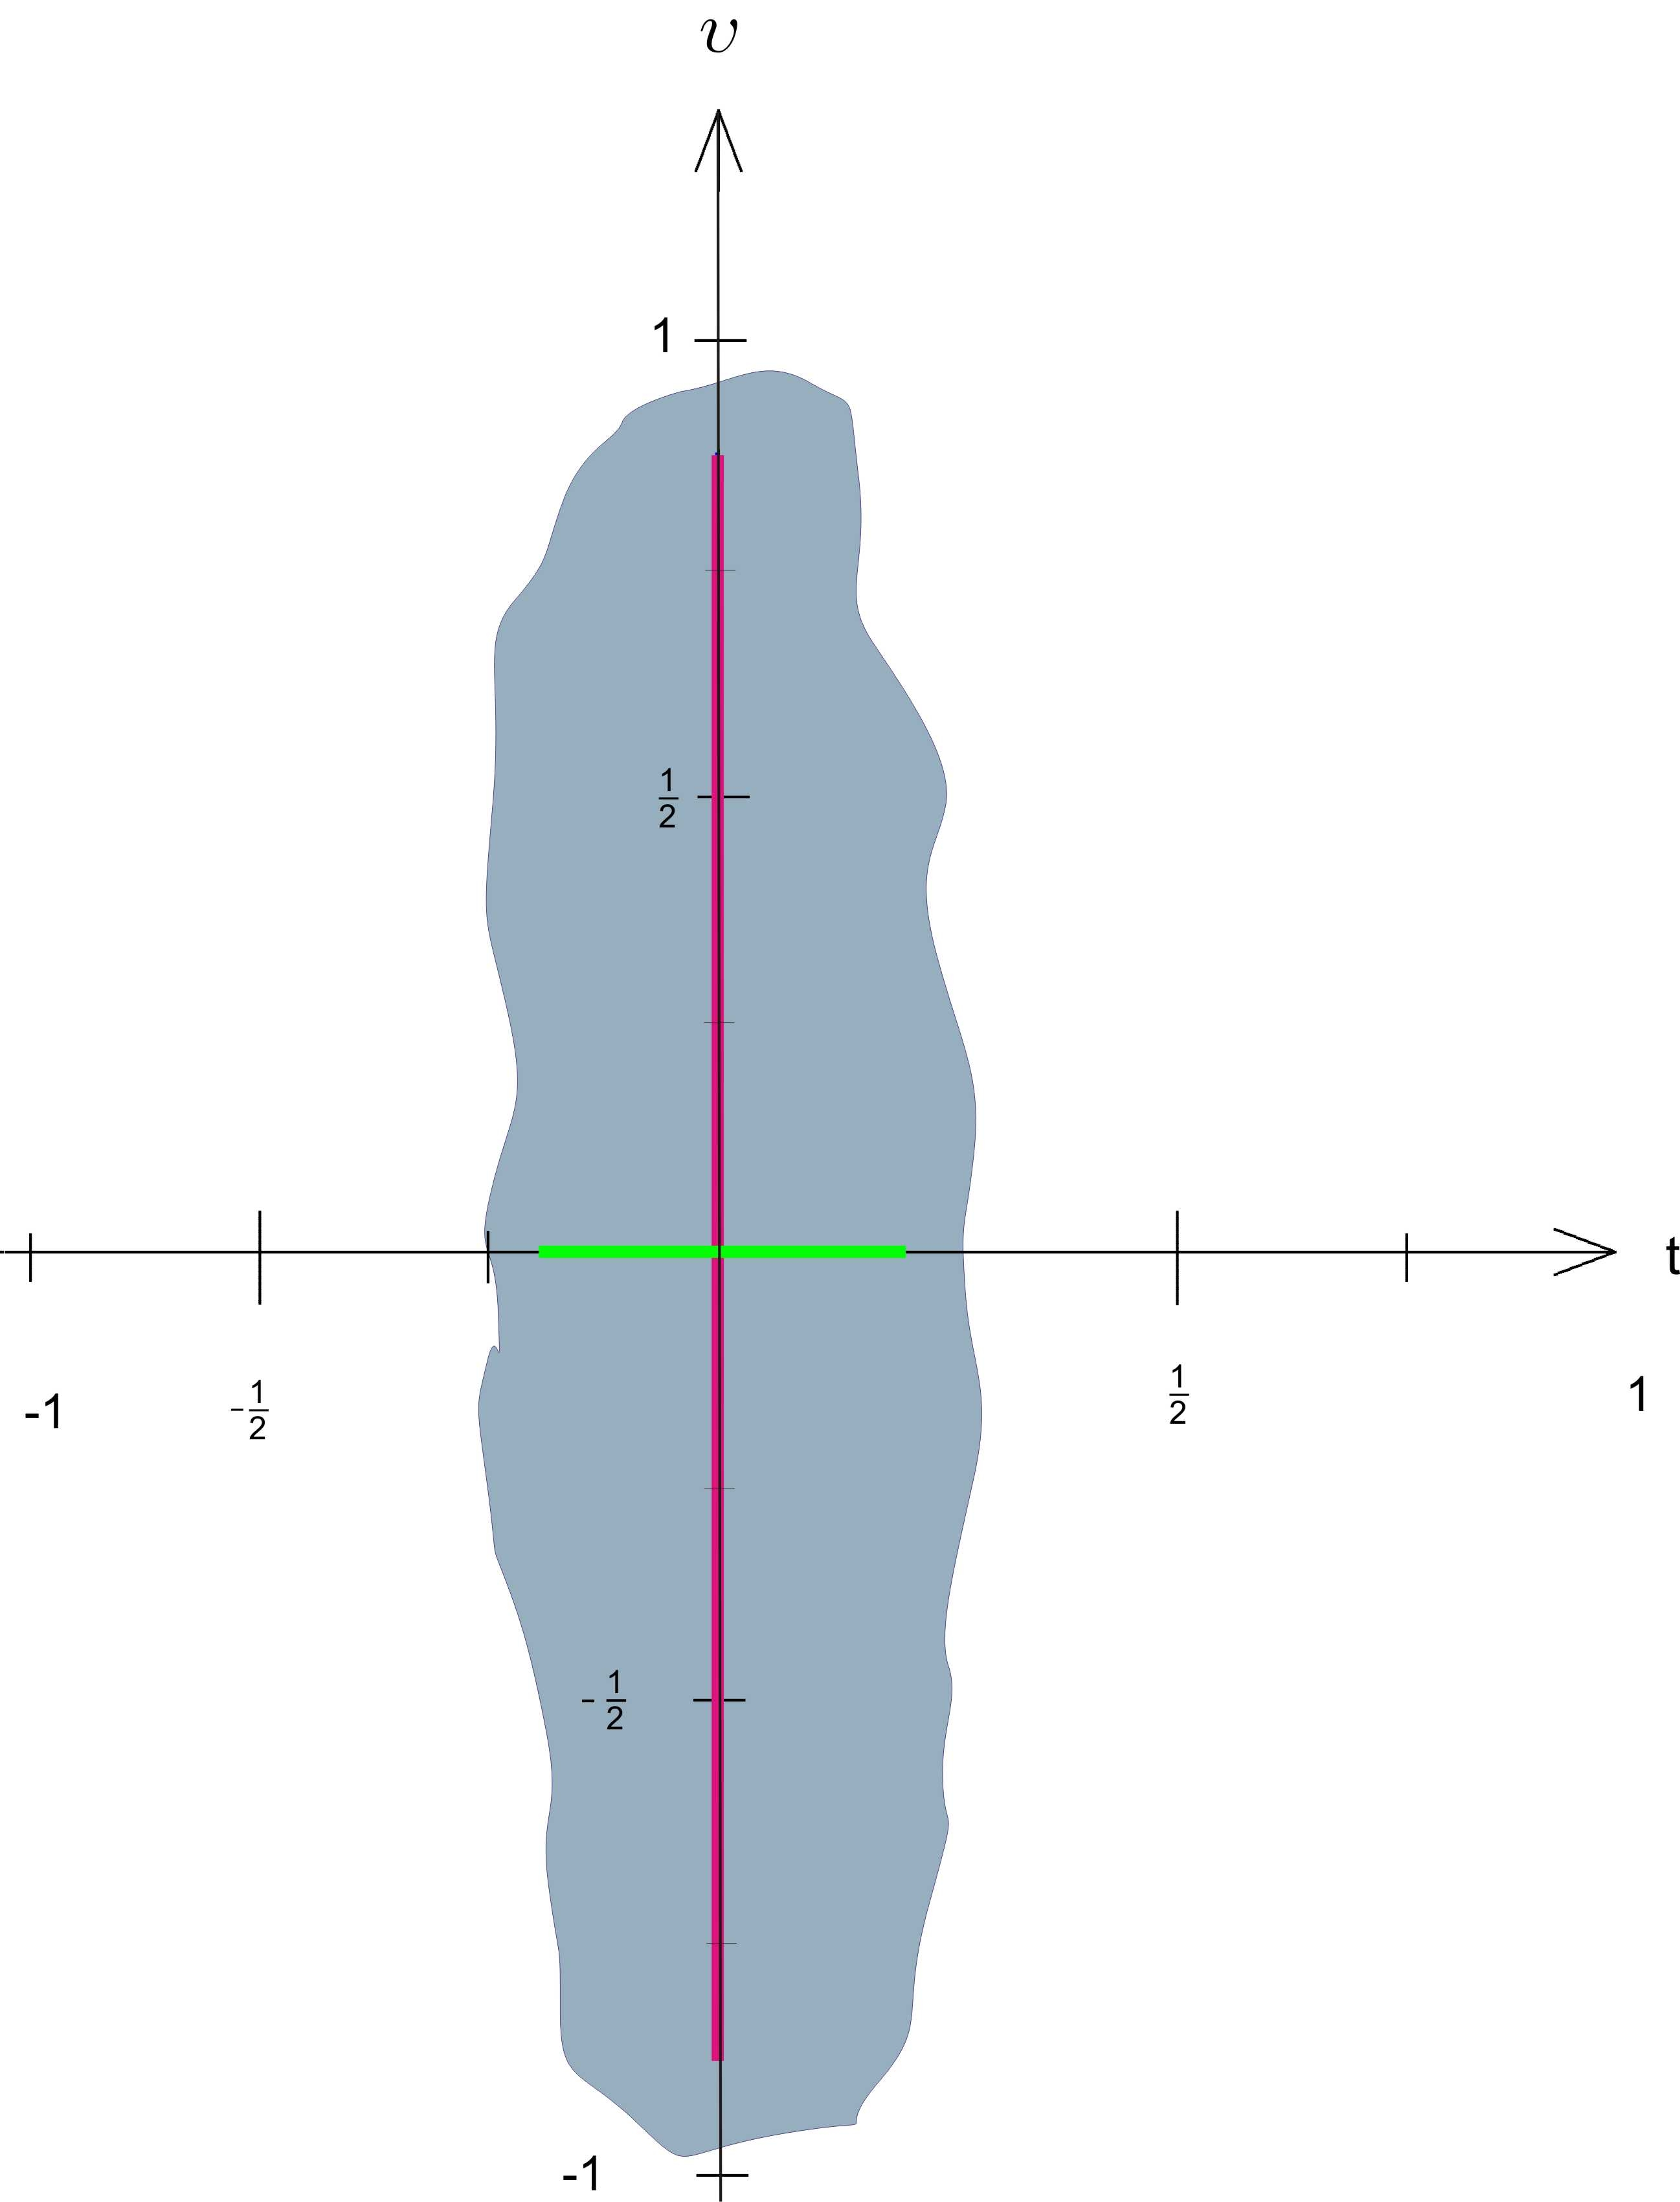
\includegraphics[width=6cm]{Pfander/pfander2.png}
    \caption{\small Our operator sampling results apply to
    all pseudodifferential operators whose Kohn--Nirenberg symbol
    is bandlimited to a Jordan domain of area less than one (e.g., the blue
    region). These results extend
    Shannon's sampling theorem which is equivalent to the identifiability of
    operators whose Kohn-Nirenberg symbol is bandlimited to a segment of the frequency shift axis (red) and
    the fact that time--invariant operators can be identified from their action on the $\delta$
    impulse. The latter holds since the Kohn--Nirenberg symbols of time--invariant operators
    are bandlimited to the time shift axis
    (green).
                }
    \label{fig:pfander2-pic-1}
  \end{center}
\end{figure}

Our results hold for a large class of operator spaces whose
definition uses the previously mentioned bandlimitation on the
Kohn-Nirenberg symbol and the flexibility of so-called modulation
spaces.  The operator spaces considered include, for example, the
identity operator, small perturbations of the identity, and
convolution operators with compactly supported kernels as examples
of identifiable operators, as well as any pseudodifferential
operator whose Kohn-Nirenberg symbol is defined on a set (Jordan
domain) of area less than one. Further, our results cover
multiplication operators with bandlimited multipliers and thereby
Shannon's sampling theorem (Fig.~\ref{fig:pfander2-pic-1}) .


% to reference it use ``Figure.~\ref{fig:xxx}''; the numbers will be computed automatically.


%
%
%which can be formulated as: A multiplication operator whose
%multiplier is bandlimited is fully represented by its action on an
%appropriately scaled Shah distribution. (The operator output are
%simply the sampling values.)



%%%%%%%%%%%%%%%%%%%%%%%%%%%%%%%%%%%%%%%%%%%%%%%%%%%%%
%%%%%%%%%%%%%%%%%%%%%%%%%%%%%%%%%%%%%%%%%%%%%%%%%%%%%
\smallskip

{\sl Uncertainty:} Heisenberg's uncertainty principle implies
that functions defined on the real line cannot be arbitrarily well
localized in time and frequency simultaneously. One of the projects
completed during 2006 considered uncertainty principles for
time-frequency representations of finite dimensional vectors, that
is, of functions defined on finite abelian groups.


In particular, we discussed  uncertainty principles for
so-called short time (or windowed) Fourier transforms. Again, the
minimum support of a short time Fourier transform equals the
dimension of the domain space and we showed that for some groups,
this well known result can be improved considerably, in particular
through the choice of an appropriate analysis window. Further, we
formulated a conjecture which relates support size constraints of
discrete Fourier transforms to support size constraints of short
time Fourier transforms \cite{KPR06}.

\medskip

  G\"otz Pfander is also involved in  ``Digital Signal Processing''
  (Section \ref{ict:pfander}).


%% to include a figure, generate a file xxx.pdf and integrate the following lines
%\begin{figure}[ht]
%  \begin{center}
%   % \includegraphics[width=10cm]{xxx}
%    \caption{The caption of the figure}
%    \label{fig:xxx}
%  \end{center}
%\end{figure}
%% to reference it use ``Figure.~\ref{fig:xxx}''; the numbers will be computed automatically.



%%%%%%%%%%%%%%%%%%%%%%%%%%%%%%%%%%%%%%%%%%%%%%%%%%%%%
%%%%%%%%%%%%%%%%%%%%%%%%%%%%%%%%%%%%%%%%%%%%%%%%%%%%%


\paragraph{Collaborations}
\begin{enumerate}

%\item {\sl International University Bremen}\\
 %Dr. Niklas Grip\\
 %Critical density in time--frequency analysis

\item {\sl Norbert Wiener Center for Harmonic Analysis and
Applications, University of Maryland, USA}\\
Consultant since 2004

\item {\sl George Mason University, USA}\\ Prof.~D. Walnut\\
Sampling of operators with bandlimited Kohn-Nirenberg symbol

\item {\sl New York University, USA}\\ F. Krahmer\\
Uncertainty principles for functions on finite groups

\item {\sl Numerical Harmonic Analysis Group and European Center for
Time-Frequency Analysis, Vienna University, Austria}\\
Prof.~H. Feichtinger, Prof.~K. Gr\"ochenig, Dr.~H. Rauhut\\
Gabor analysis and applications to mobile communications, sparse
representations

\end{enumerate}


%%%%%%%%%%%%%%%%%%%%%%%%%%%%%%%%%%%%%%%%%%%%%%%%%%%%%
%%%%%%%%%%%%%%%%%%%%%%%%%%%%%%%%%%%%%%%%%%%%%%%%%%%%%

\paragraph{Grants}
% list the running grants in 2005, if none have been received, please delete this
% subsection.
\begin{enumerate}
\item Funded by DFG, \emph{Analysis and design of COFDM
multicarrier modulation techniques in view of transmission
stability in time variant channels,} within the DFG priority
program 1163.

\item  Funded by DFG, \emph{Travel grant: International Conference Harmonic Analysis and
    Applications, Merlo, Argentina}. 

\item  Funded by DAAD, \emph{Full fellowship for Peter Rashkov to work on the PhD topic
    ''Smooth Gabor frames for arbitrary lattices''}
\end{enumerate}


%%%%%%%%%%%%%%%%%%%%%%%%%%%%%%%%%%%%%%%%%%%%%%%%%%%%%
%%%%%%%%%%%%%%%%%%%%%%%%%%%%%%%%%%%%%%%%%%%%%%%%%%%%%

%\paragraph{Publications}
% list the publications of 2005 (also accepted and in press), if none have been received, plese delete this
% subsection. Enter the publications into the SES publications database at
% http://kwarc.eecs.iu-bremen.de/ses-pubs/index.php and only reference them here.

%\begin{description}
 %   \item[Journals] Journal of Fourier Analysis and
 %   Applications~

  %  Applied and Computational
   % Analysis~
    \nocite{BP06}
    %, SIAM Journal of Mathematical
    %Analysis~
    \nocite{KP06} %Sampling Theory in Signal and Image
    %Processing~
    \nocite{PW06}
    \nocite{GP06}
%\end{description}
